\section{Analysis}\label{sec:analysis}

\subsection{Training samples}
The signal window is defined as the shortest interval that contains $\SI{99}{\percent}$ of the simulated $B^0_s$ decays as shown in \autoref{fig:Bs_sim}.
It is found to be $\SIrange{5333}{5395}{\mega\eV}$ and will be needed to determine the number of signal events at the very end of this analysis.

\begin{figure}[H]
  \centering
  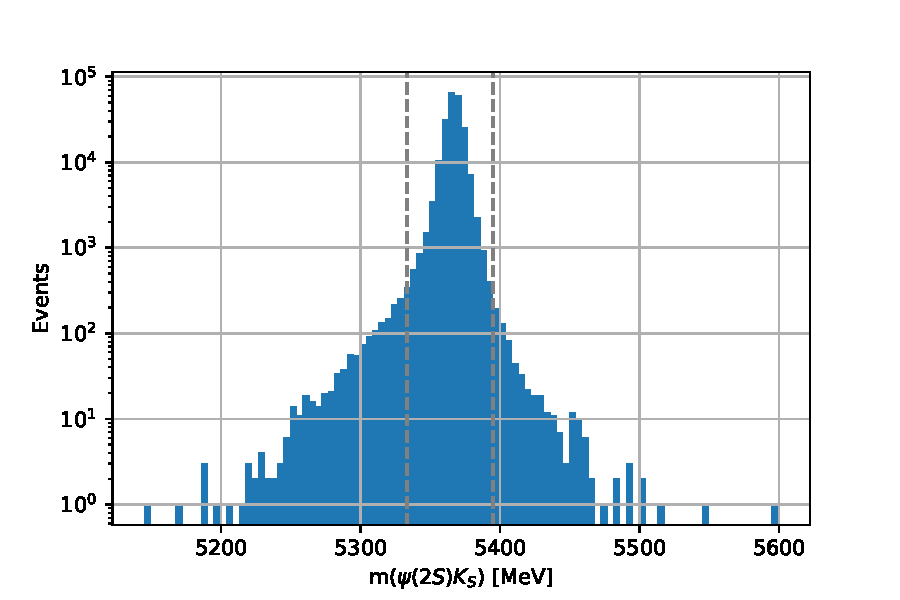
\includegraphics[width=12cm]{plots/sim_hist_limits.pdf}
  \caption{Invariant mass distribution of the decay products of the MC simulated decay $B^0_s \to \psi(2S)K^0_\mathrm{S}$ (blue bars) with upper and lower limit of the signal region (gray dashed lines).}
  \label{fig:Bs_sim}
\end{figure}

The $B^0_s$ MC also acts as signal training sample for the upcoming classification. As background training sample the upper sideband (USB) of the recorded data is used, which is all recorded data with a reconstructed invariant mass higher than the highest simulated invariant mass. In this region the data is expected to mainly consist of combinatorial background.

\subsection{Feature selection}
For the classification over $\num{800}$ features are available, but using all of these would result in a really long computation time and also not all of these features are simulated perfectly. Therefore these need to be reduced significantly.

As a first step features are rejected that are poorly described by the simulation. Using these features would result in a classification between data and simulation instead of signal and background. To locate these features the Kolmogorov-Smirnov test is used which compares two cumulative probability distributions $F^i$ with the distance

\begin{equation*}
  d = \sup_x \left|F^1(x) - F^2(x)\right|.
\end{equation*}

In this first step the distributions of each feature of the $B^0_d$ MC are compared to those of the sWeighted data sample as shown in \autoref{fig:sWeights}. These sWeights are obtained from a so called sPlot, which is a statistical method to extract one component from data with various components, in this case possible $B^0_d$ candidates. To the $B^0_d$ MC, kinematic weights are applied to make up partially for features that are not simulated flawlessly. It is expected that the simulations act similarly for $B^0_d$ and $B^0_s$, but the latter cannot be seen in data due to the large background. Therefore the comparison of each feature in data and simulation is done with $B^0_d$.

\begin{figure}[H]
  \centering
  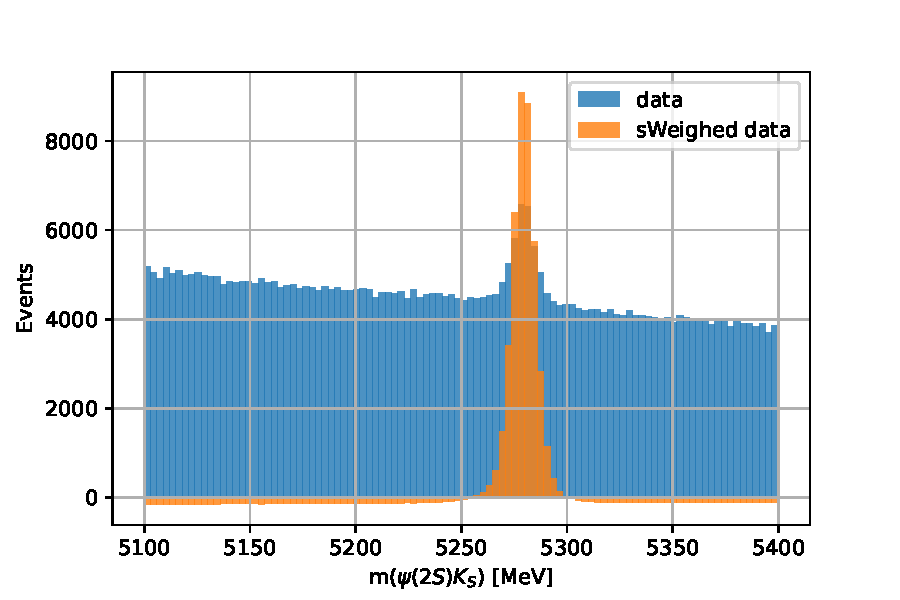
\includegraphics[width=12cm]{plots/sweights.pdf}
  \caption{Invariant mass distribution of data measured by the LHCb experiment without (blue) and with (orange) sWeights applied to extract $B^0_d$ candidates.}
  \label{fig:sWeights}
\end{figure}

In the next step, the $\num{100}$ most similar features in data and simulation are considered. Here, features that are distributed similarly in the $B^0_s$ simulation and the USB of the data are rejected, because they do not help the classification, but only slow down the computation. The distributions are compared with the same metric as before and the $\num{10}$ features with the lowest similarity are taken into account for the classifier.

As a last step it is checked that these features are not highly correlated with the invariant $B^0_s$ mass. To do so, the Pearson correlation coefficient is computed for each of the chosen features with the invariant mass. None of the chosen features are highly correlated.

\subsection{Multivariate classification}
The XGBoost classifier~\cite{Chen:2016:XST:2939672.2939785} is used as a multivariate classifier to differentiate between signal and background. It is provided the features selected in the last section for training. Since there is much more bakckground ind the training data it is weighted so that the classifier is trained equally on signal and background. To prevent overfitting and bias in training a $k$-fold is applied. The data is split into $k$ parts and $k$ BDTs are trained on $k - 1$ subsets while the remaining subset is used for validation. This method also has the advantage that no data is only used for validating the classifier. In this analysis a $k$-fold is applied with $k = 5$.

The performance of the BDTs is studied using a receiver operating characteristics (ROC) curve. It shows the true positive rate (TPR) of a classifier as a function of its false positive rate (FPR), corresponding to different cut values on the classifier's output. It can be evaluated with the area under the ROC curve (AUC) which equals $1$ for a perfect classifier and $0.5$ for a randomly guessing classifier. The mean ROC curve for the classifier used in this analysis is shown in \autoref{fig:roc}. It can be seen that each BDT ROC curves merely differ from the mean ROC curve, proving that there is no bias or overfitting issues. The AUC score of $\num{0.98 \pm 0.0003}$ confirms the good performance of the classifier.

\begin{figure}[tb]
  \centering
  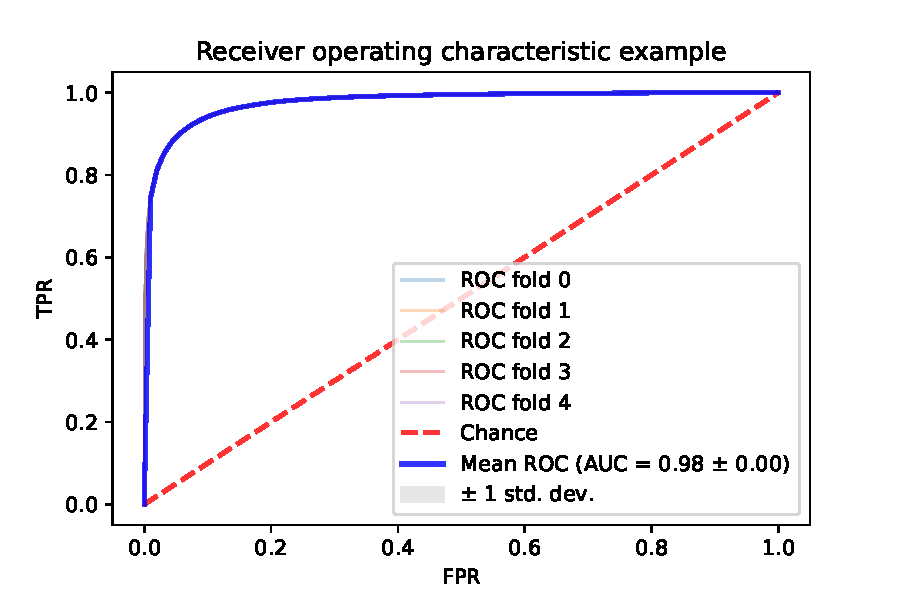
\includegraphics[width=.8\textwidth]{plots/roc.pdf}
  \caption{Mean ROC curve for the classifier trained for this analysis with one standard deviation and ROC curves for each BDT.}
  \label{fig:roc}
\end{figure}

To determine the best possible cut on the classifier the Punzi Figure of Merit (FOM)
\begin{equation*}
  \mathrm{FOM} = \frac{\epsilon_\mathrm{sig}}{\frac{5}{2} + \sqrt{N_\mathrm{bkg}}}
\end{equation*}
with the signal efficiency $\epsilon_\mathrm{sig}$ and the number of background events in the signal region $N_\mathrm{bkg}$ is used as a metric. The Punzi FOM quantizes the tradeoff between background rejection and conservation of signal and it is not dependent on the absolute number of signal candidates which is perfect in the case of polluted data samples like this one.
To obtain the signal efficiency, the number of candidates before and after the BDT cut are compared in the signal simulation. For $N_\mathrm{bkg}$ it is assumed that the background efficiency is constant and therefore obtained from the USB. In the signal region it is assumed that the signal contribution is negligible in comparison to the background.
The Punzi FOM is shown in \autoref{fig:punzi} and the optimal cut value is found to be $\num{0.995}$.

\begin{figure}[tb]
  \centering
  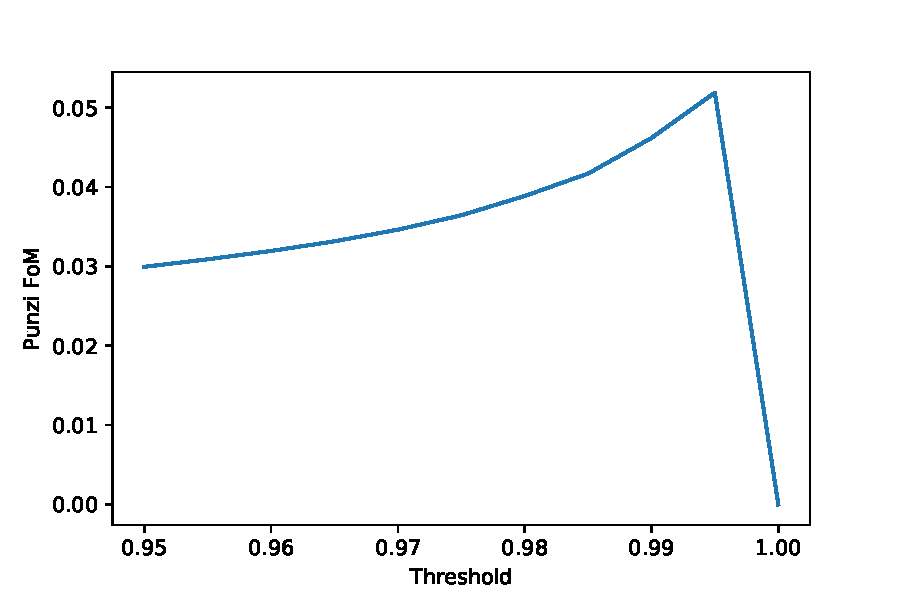
\includegraphics[width=.8\textwidth]{plots/FoM.pdf}
  \caption{Punzi FOM as a function of the cut value on the mean BDT output.}
  \label{fig:punzi}
\end{figure}

The invariant mass distribution after applying the BDT cut is shown in \autoref{fig:mass_cut}. It shows a clrarly visible $B^0_d$ peak and a small $B^0_s$ peak polluted with a remaining, but significantly smaller combinatorial background. To evaluate the $B^0_s$ peak fits need to be made on the distribution.

\begin{figure}[tb]
  \centering
  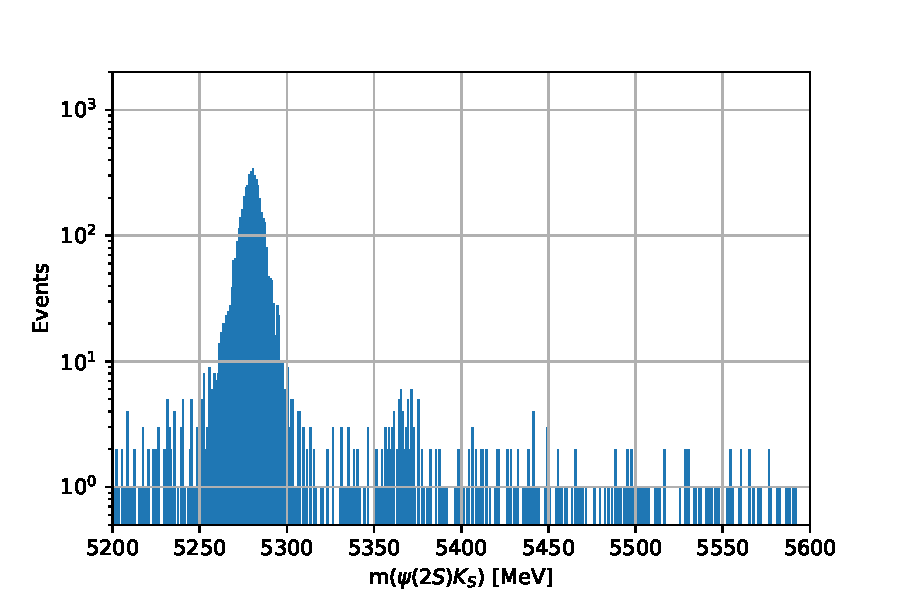
\includegraphics[width=.8\textwidth]{plots/signal_window_cut.pdf}
  \caption{Invariant mass distribution after applying the BDT cut.}
  \label{fig:mass_cut}
\end{figure}

\subsection{Invariant mass fit}
The fit model used in this analysis consists of three components: the $B^0_s$ peak and the $B^0_d$ peaks, each modeled by the sum of two Gaussian distributions, and the combinatorial background, modeled by an exponential function. The parameters for the two peak models are obtained by fits to the corresponding MC simulation. For the $B^0_s$ fit the obtained parameters are
\begin{align*}
  &\mu_{1, B^0_s} = \SI{5367.16 \pm 0.03}{\mega\eV} && \mu_{2, B^0_s} = \SI{5359.9 \pm 0.92}{\mega\eV}\\
  &\sigma_{1, B^0_s} = \num{5.41 \pm 0.042} && \sigma_{2, B^0_s} = \num{27.8 \pm 2.1}\\
  &\mathrm{frac}_{B^0_s} = \num{0.939 \pm 0.0031}
\end{align*}
and for the $B^0_d$ fit the parameters
\begin{align*}
  &\mu_{1, B^0_d} = \SI{5275.0 \pm 0.35}{\mega\eV} && \mu_{2, B^0_d} = \SI{5279.94 \pm 0.035}{\mega\eV}\\
  &\sigma_{1, B^0_d} = \num{19.8 \pm 0.46} && \sigma_{2, B^0_d} = \num{4.97 \pm 0.039}\\
  &\mathrm{frac}_{B^0_d} = \num{0.0870 \pm 0.0042}
\end{align*}
are obtained.

\begin{figure}[tb]
  \centering
  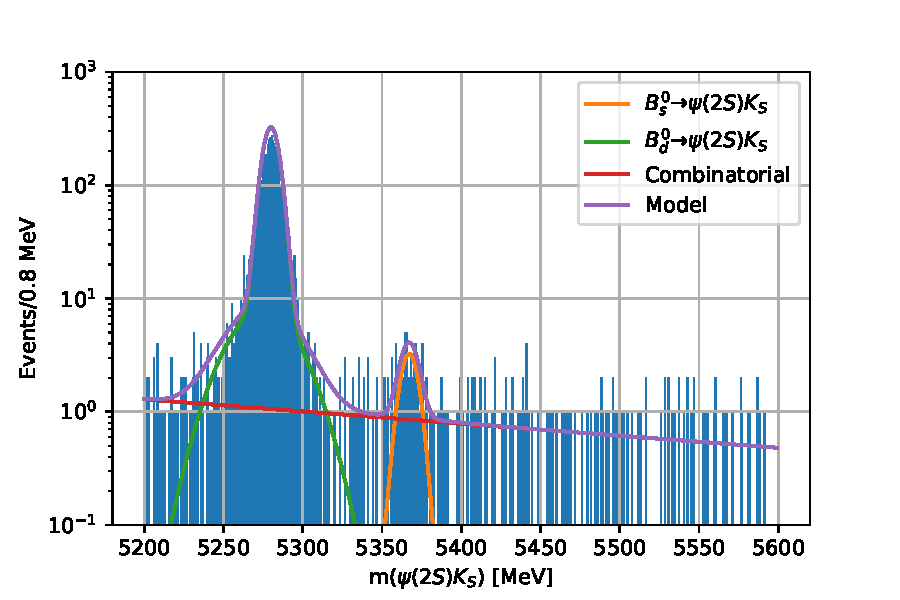
\includegraphics[width=12cm]{plots/data_fit_extended.pdf}
  \caption{Extended fit (purple) to the selected invariant mass spectrum of $\psi(2S)$ and $K^0_\mathrm{S}$ (blue bars). Also shown are the submodels for $B^0_d \to \psi(2S)K^0_\mathrm{S}$ (green), $B^0_s \to \psi(2S)K^0_\mathrm{S}$ (orange), and the combinatorial background model (red).}
  \label{fig:model}
\end{figure}

These are fixed for the fit of the full model to the selected data. It consists of the sum of the two peak models and the exponential function with a decay constant $\lambda_\mathrm{bkg}$ modelling the combinatorial background, each multiplied by their respective yield in the fit window. The fit is shown in \autoref{fig:model} and the obtained values for the free parameters are
\begin{align*}
  &\lambda_\mathrm{bkg} = \SI{0.0025 \pm 0.00057}{\per\mega\eV} && N_{B^0_s} = \num{46 \pm 8.5}\\
  &N_{B^0_d} = \num{4330 \pm 67} && N_\mathrm{comb} = \num{330 \pm 23}.
\end{align*}

To estimate the statistical significance of this result the significance proxy
\begin{equation*}
  m = \frac{n_\mathrm{sig}}{\sqrt{n_\mathrm{sig} + n_\mathrm{bkg}}}
\end{equation*}
is used, where $n_\mathrm{sig}$ and $n_\mathrm{bkg}$ are the observed numbers of signal and background events in the signal region, respectively. To obtain these one needs to integrate the extended PDFs over the signal window.
The numbers of observed signal and background events in the signal region are found to be $n_\mathrm{sig} = \num{45.61}$ and $n_\mathrm{bkg} = \num{53.34}$, corresponding to a statistical significance proxy $m =\num{4.6}\sigma$.
